\begin{figure}[h]
\begin{center}
\begin{adjustbox}{width=\columnwidth}
    \tikzset{every picture/.style={line width=0.75pt}} %set default line width to 0.75pt        
    
    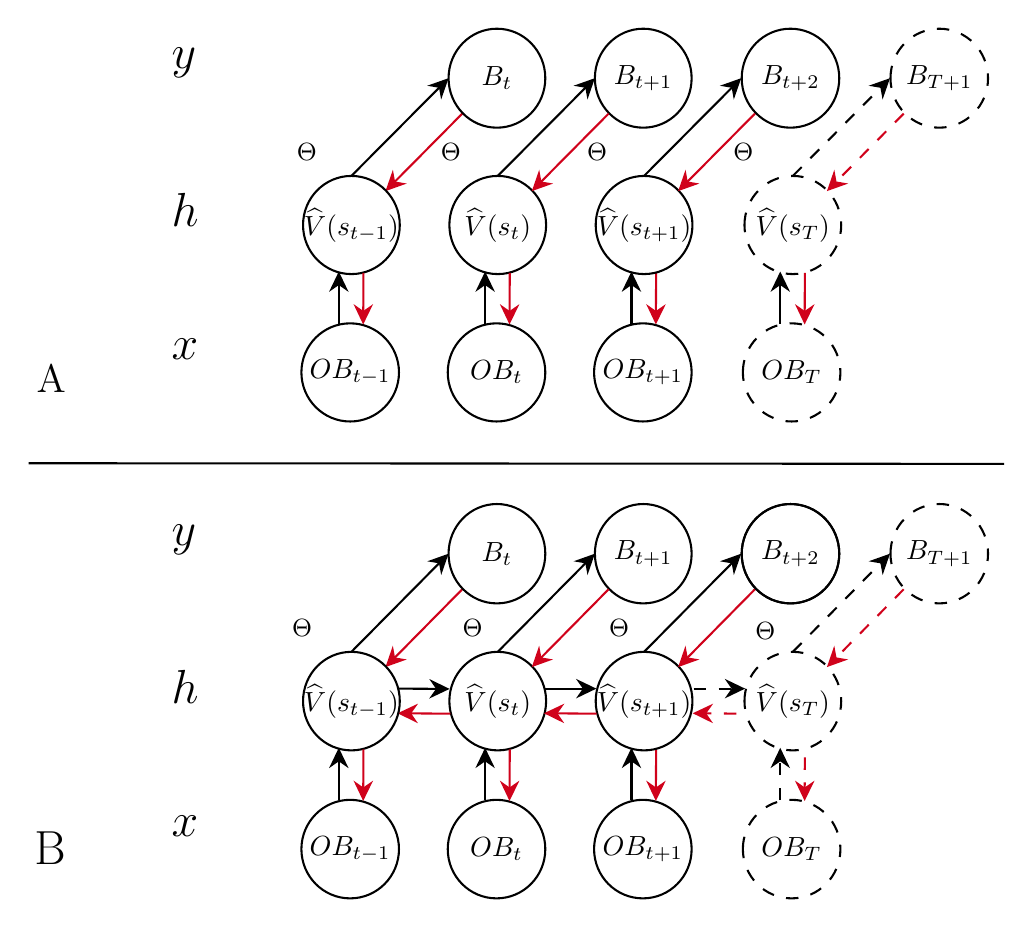
\begin{tikzpicture}[x=0.75pt,y=0.75pt,yscale=-1,xscale=1]
    %uncomment if require: \path (0,432); %set diagram left start at 0, and has height of 432
    
    %Shape: Ellipse [id:dp9152556376471453] 
    \draw   (252.87,325.26) .. controls (252.87,312.15) and (263.3,301.52) .. (276.18,301.52) .. controls (289.05,301.52) and (299.48,312.15) .. (299.48,325.26) .. controls (299.48,338.37) and (289.05,349) .. (276.18,349) .. controls (263.3,349) and (252.87,338.37) .. (252.87,325.26) -- cycle ;
    %Straight Lines [id:da0084456304461753] 
    \draw [color={rgb, 255:red, 208; green, 2; blue, 27 }  ,draw opacity=1 ]   (230.94,331.15) -- (253.32,331.31) ;
    \draw [shift={(227.94,331.12)}, rotate = 0.43] [fill={rgb, 255:red, 208; green, 2; blue, 27 }  ,fill opacity=1 ][line width=0.08]  [draw opacity=0] (9.82,-4.72) -- (0,0) -- (9.82,4.72) -- (6.52,0) -- cycle    ;
    %Shape: Ellipse [id:dp18326344407352502] 
    \draw   (181.58,396.56) .. controls (181.58,383.45) and (192.11,372.82) .. (205.08,372.82) .. controls (218.06,372.82) and (228.59,383.45) .. (228.59,396.56) .. controls (228.59,409.67) and (218.06,420.3) .. (205.08,420.3) .. controls (192.11,420.3) and (181.58,409.67) .. (181.58,396.56) -- cycle ;
    %Shape: Ellipse [id:dp4732045107682973] 
    \draw   (252.09,396.56) .. controls (252.09,383.45) and (262.61,372.82) .. (275.59,372.82) .. controls (288.57,372.82) and (299.09,383.45) .. (299.09,396.56) .. controls (299.09,409.67) and (288.57,420.3) .. (275.59,420.3) .. controls (262.61,420.3) and (252.09,409.67) .. (252.09,396.56) -- cycle ;
    %Straight Lines [id:da9106304988340169] 
    \draw    (205.67,301.52) -- (250.37,256.37) ;
    \draw [shift={(252.48,254.24)}, rotate = 494.71] [fill={rgb, 255:red, 0; green, 0; blue, 0 }  ][line width=0.08]  [draw opacity=0] (9.82,-4.72) -- (0,0) -- (9.82,4.72) -- (6.52,0) -- cycle    ;
    %Straight Lines [id:da5186602107869037] 
    \draw [color={rgb, 255:red, 208; green, 2; blue, 27 }  ,draw opacity=1 ]   (259.09,271.36) -- (224.2,306.73) ;
    \draw [shift={(222.1,308.86)}, rotate = 314.62] [fill={rgb, 255:red, 208; green, 2; blue, 27 }  ,fill opacity=1 ][line width=0.08]  [draw opacity=0] (9.82,-4.72) -- (0,0) -- (9.82,4.72) -- (6.52,0) -- cycle    ;
    %Shape: Ellipse [id:dp6434768624828036] 
    \draw   (322.59,396.56) .. controls (322.59,383.45) and (333.11,372.82) .. (346.09,372.82) .. controls (359.07,372.82) and (369.59,383.45) .. (369.59,396.56) .. controls (369.59,409.67) and (359.07,420.3) .. (346.09,420.3) .. controls (333.11,420.3) and (322.59,409.67) .. (322.59,396.56) -- cycle ;
    %Shape: Ellipse [id:dp4847846412537088] 
    \draw   (252.48,254.24) .. controls (252.48,241.02) and (262.91,230.3) .. (275.78,230.3) .. controls (288.65,230.3) and (299.09,241.02) .. (299.09,254.24) .. controls (299.09,267.46) and (288.65,278.18) .. (275.78,278.18) .. controls (262.91,278.18) and (252.48,267.46) .. (252.48,254.24) -- cycle ;
    %Shape: Ellipse [id:dp07973567399208026] 
    \draw   (322.98,254.24) .. controls (322.98,241.02) and (333.42,230.3) .. (346.29,230.3) .. controls (359.16,230.3) and (369.59,241.02) .. (369.59,254.24) .. controls (369.59,267.46) and (359.16,278.18) .. (346.29,278.18) .. controls (333.42,278.18) and (322.98,267.46) .. (322.98,254.24) -- cycle ;
    %Shape: Ellipse [id:dp05423142626898558] 
    \draw   (393.72,254.24) .. controls (393.72,241.02) and (404.24,230.3) .. (417.22,230.3) .. controls (430.2,230.3) and (440.72,241.02) .. (440.72,254.24) .. controls (440.72,267.46) and (430.2,278.18) .. (417.22,278.18) .. controls (404.24,278.18) and (393.72,267.46) .. (393.72,254.24) -- cycle ;
    %Shape: Ellipse [id:dp22782348689960996] 
    \draw   (182.37,325.26) .. controls (182.37,312.15) and (192.8,301.52) .. (205.67,301.52) .. controls (218.54,301.52) and (228.98,312.15) .. (228.98,325.26) .. controls (228.98,338.37) and (218.54,349) .. (205.67,349) .. controls (192.8,349) and (182.37,338.37) .. (182.37,325.26) -- cycle ;
    %Straight Lines [id:da8044112442211012] 
    \draw [line width=0.75]    (270.1,372.91) -- (270.1,350.76) ;
    \draw [shift={(270.1,347.76)}, rotate = 450] [fill={rgb, 255:red, 0; green, 0; blue, 0 }  ][line width=0.08]  [draw opacity=0] (9.82,-4.72) -- (0,0) -- (9.82,4.72) -- (6.52,0) -- cycle    ;
    %Straight Lines [id:da4352361095595384] 
    \draw [color={rgb, 255:red, 208; green, 2; blue, 27 }  ,draw opacity=1 ]   (281.87,370.38) -- (281.97,348.47) ;
    \draw [shift={(281.85,373.38)}, rotate = 270.27] [fill={rgb, 255:red, 208; green, 2; blue, 27 }  ,fill opacity=1 ][line width=0.08]  [draw opacity=0] (9.82,-4.72) -- (0,0) -- (9.82,4.72) -- (6.52,0) -- cycle    ;
    %Straight Lines [id:da9840961706533492] 
    \draw [color={rgb, 255:red, 0; green, 0; blue, 0 }  ,draw opacity=1 ]   (228.41,319.25) -- (249.98,319.36) ;
    \draw [shift={(252.98,319.38)}, rotate = 180.28] [fill={rgb, 255:red, 0; green, 0; blue, 0 }  ,fill opacity=1 ][line width=0.08]  [draw opacity=0] (9.82,-4.72) -- (0,0) -- (9.82,4.72) -- (6.52,0) -- cycle    ;
    %Straight Lines [id:da9105454079139469] 
    \draw [line width=0.75]    (340.61,372.91) -- (340.61,350.76) ;
    \draw [shift={(340.61,347.76)}, rotate = 450] [fill={rgb, 255:red, 0; green, 0; blue, 0 }  ][line width=0.08]  [draw opacity=0] (9.82,-4.72) -- (0,0) -- (9.82,4.72) -- (6.52,0) -- cycle    ;
    %Straight Lines [id:da2563913907740285] 
    \draw [color={rgb, 255:red, 208; green, 2; blue, 27 }  ,draw opacity=1 ]   (352.37,370.38) -- (352.48,348.47) ;
    \draw [shift={(352.36,373.38)}, rotate = 270.27] [fill={rgb, 255:red, 208; green, 2; blue, 27 }  ,fill opacity=1 ][line width=0.08]  [draw opacity=0] (9.82,-4.72) -- (0,0) -- (9.82,4.72) -- (6.52,0) -- cycle    ;
    %Shape: Ellipse [id:dp3682545800349367] 
    \draw   (323.37,325.26) .. controls (323.37,312.15) and (333.81,301.52) .. (346.68,301.52) .. controls (359.55,301.52) and (369.98,312.15) .. (369.98,325.26) .. controls (369.98,338.37) and (359.55,349) .. (346.68,349) .. controls (333.81,349) and (323.37,338.37) .. (323.37,325.26) -- cycle ;
    %Straight Lines [id:da5491729665822646] 
    \draw [line width=0.75]    (199.6,372.91) -- (199.6,350.76) ;
    \draw [shift={(199.6,347.76)}, rotate = 450] [fill={rgb, 255:red, 0; green, 0; blue, 0 }  ][line width=0.08]  [draw opacity=0] (9.82,-4.72) -- (0,0) -- (9.82,4.72) -- (6.52,0) -- cycle    ;
    %Straight Lines [id:da6906936296691885] 
    \draw [color={rgb, 255:red, 208; green, 2; blue, 27 }  ,draw opacity=1 ]   (211.37,370.38) -- (211.47,348.47) ;
    \draw [shift={(211.35,373.38)}, rotate = 270.27] [fill={rgb, 255:red, 208; green, 2; blue, 27 }  ,fill opacity=1 ][line width=0.08]  [draw opacity=0] (9.82,-4.72) -- (0,0) -- (9.82,4.72) -- (6.52,0) -- cycle    ;
    %Straight Lines [id:da8976403312606693] 
    \draw [color={rgb, 255:red, 208; green, 2; blue, 27 }  ,draw opacity=1 ]   (301.45,331.15) -- (323.82,331.31) ;
    \draw [shift={(298.45,331.12)}, rotate = 0.43] [fill={rgb, 255:red, 208; green, 2; blue, 27 }  ,fill opacity=1 ][line width=0.08]  [draw opacity=0] (9.82,-4.72) -- (0,0) -- (9.82,4.72) -- (6.52,0) -- cycle    ;
    %Straight Lines [id:da7873502214297404] 
    \draw [color={rgb, 255:red, 0; green, 0; blue, 0 }  ,draw opacity=1 ]   (298.92,319.25) -- (320.69,319.25) ;
    \draw [shift={(323.69,319.25)}, rotate = 180] [fill={rgb, 255:red, 0; green, 0; blue, 0 }  ,fill opacity=1 ][line width=0.08]  [draw opacity=0] (9.82,-4.72) -- (0,0) -- (9.82,4.72) -- (6.52,0) -- cycle    ;
    %Straight Lines [id:da38615546041268245] 
    \draw    (276.18,301.52) -- (320.87,256.37) ;
    \draw [shift={(322.98,254.24)}, rotate = 494.71] [fill={rgb, 255:red, 0; green, 0; blue, 0 }  ][line width=0.08]  [draw opacity=0] (9.82,-4.72) -- (0,0) -- (9.82,4.72) -- (6.52,0) -- cycle    ;
    %Straight Lines [id:da8727709104298054] 
    \draw [color={rgb, 255:red, 208; green, 2; blue, 27 }  ,draw opacity=1 ]   (329.6,271.36) -- (294.71,306.73) ;
    \draw [shift={(292.6,308.86)}, rotate = 314.62] [fill={rgb, 255:red, 208; green, 2; blue, 27 }  ,fill opacity=1 ][line width=0.08]  [draw opacity=0] (9.82,-4.72) -- (0,0) -- (9.82,4.72) -- (6.52,0) -- cycle    ;
    %Straight Lines [id:da025606451942667974] 
    \draw    (346.68,301.52) -- (391.37,256.37) ;
    \draw [shift={(393.48,254.24)}, rotate = 494.71] [fill={rgb, 255:red, 0; green, 0; blue, 0 }  ][line width=0.08]  [draw opacity=0] (9.82,-4.72) -- (0,0) -- (9.82,4.72) -- (6.52,0) -- cycle    ;
    %Straight Lines [id:da7157498693904918] 
    \draw [color={rgb, 255:red, 208; green, 2; blue, 27 }  ,draw opacity=1 ]   (400.1,271.36) -- (365.21,306.73) ;
    \draw [shift={(363.1,308.86)}, rotate = 314.62] [fill={rgb, 255:red, 208; green, 2; blue, 27 }  ,fill opacity=1 ][line width=0.08]  [draw opacity=0] (9.82,-4.72) -- (0,0) -- (9.82,4.72) -- (6.52,0) -- cycle    ;
    %Shape: Ellipse [id:dp1944088973906778] 
    \draw   (252.87,95.88) .. controls (252.87,82.82) and (263.3,72.23) .. (276.18,72.23) .. controls (289.05,72.23) and (299.48,82.82) .. (299.48,95.88) .. controls (299.48,108.94) and (289.05,119.52) .. (276.18,119.52) .. controls (263.3,119.52) and (252.87,108.94) .. (252.87,95.88) -- cycle ;
    %Shape: Ellipse [id:dp7540301212468546] 
    \draw   (181.58,166.89) .. controls (181.58,153.83) and (192.11,143.25) .. (205.08,143.25) .. controls (218.06,143.25) and (228.59,153.83) .. (228.59,166.89) .. controls (228.59,179.95) and (218.06,190.54) .. (205.08,190.54) .. controls (192.11,190.54) and (181.58,179.95) .. (181.58,166.89) -- cycle ;
    %Shape: Ellipse [id:dp5780436923676984] 
    \draw   (252.09,166.89) .. controls (252.09,153.83) and (262.61,143.25) .. (275.59,143.25) .. controls (288.57,143.25) and (299.09,153.83) .. (299.09,166.89) .. controls (299.09,179.95) and (288.57,190.54) .. (275.59,190.54) .. controls (262.61,190.54) and (252.09,179.95) .. (252.09,166.89) -- cycle ;
    %Straight Lines [id:da6776717368806907] 
    \draw    (205.67,72.23) -- (250.36,27.27) ;
    \draw [shift={(252.48,25.14)}, rotate = 494.83] [fill={rgb, 255:red, 0; green, 0; blue, 0 }  ][line width=0.08]  [draw opacity=0] (9.82,-4.72) -- (0,0) -- (9.82,4.72) -- (6.52,0) -- cycle    ;
    %Straight Lines [id:da030655313121066063] 
    \draw [color={rgb, 255:red, 208; green, 2; blue, 27 }  ,draw opacity=1 ]   (259.09,42.2) -- (224.21,77.42) ;
    \draw [shift={(222.1,79.55)}, rotate = 314.73] [fill={rgb, 255:red, 208; green, 2; blue, 27 }  ,fill opacity=1 ][line width=0.08]  [draw opacity=0] (9.82,-4.72) -- (0,0) -- (9.82,4.72) -- (6.52,0) -- cycle    ;
    %Shape: Ellipse [id:dp9167477381870462] 
    \draw   (322.59,166.89) .. controls (322.59,153.83) and (333.11,143.25) .. (346.09,143.25) .. controls (359.07,143.25) and (369.59,153.83) .. (369.59,166.89) .. controls (369.59,179.95) and (359.07,190.54) .. (346.09,190.54) .. controls (333.11,190.54) and (322.59,179.95) .. (322.59,166.89) -- cycle ;
    %Shape: Ellipse [id:dp28076940126490224] 
    \draw   (252.48,25.14) .. controls (252.48,11.97) and (262.91,1.3) .. (275.78,1.3) .. controls (288.65,1.3) and (299.09,11.97) .. (299.09,25.14) .. controls (299.09,38.31) and (288.65,48.98) .. (275.78,48.98) .. controls (262.91,48.98) and (252.48,38.31) .. (252.48,25.14) -- cycle ;
    %Shape: Ellipse [id:dp018136489069107253] 
    \draw   (322.98,25.14) .. controls (322.98,11.97) and (333.42,1.3) .. (346.29,1.3) .. controls (359.16,1.3) and (369.59,11.97) .. (369.59,25.14) .. controls (369.59,38.31) and (359.16,48.98) .. (346.29,48.98) .. controls (333.42,48.98) and (322.98,38.31) .. (322.98,25.14) -- cycle ;
    %Shape: Ellipse [id:dp43337791741971476] 
    \draw   (393.72,25.14) .. controls (393.72,11.97) and (404.24,1.3) .. (417.22,1.3) .. controls (430.2,1.3) and (440.72,11.97) .. (440.72,25.14) .. controls (440.72,38.31) and (430.2,48.98) .. (417.22,48.98) .. controls (404.24,48.98) and (393.72,38.31) .. (393.72,25.14) -- cycle ;
    %Shape: Ellipse [id:dp27462372888763276] 
    \draw   (182.37,95.88) .. controls (182.37,82.82) and (192.8,72.23) .. (205.67,72.23) .. controls (218.54,72.23) and (228.98,82.82) .. (228.98,95.88) .. controls (228.98,108.94) and (218.54,119.52) .. (205.67,119.52) .. controls (192.8,119.52) and (182.37,108.94) .. (182.37,95.88) -- cycle ;
    %Straight Lines [id:da29813692702208516] 
    \draw [line width=0.75]    (270.1,143.33) -- (270.1,121.29) ;
    \draw [shift={(270.1,118.29)}, rotate = 450] [fill={rgb, 255:red, 0; green, 0; blue, 0 }  ][line width=0.08]  [draw opacity=0] (9.82,-4.72) -- (0,0) -- (9.82,4.72) -- (6.52,0) -- cycle    ;
    %Straight Lines [id:da3349478757051123] 
    \draw [color={rgb, 255:red, 208; green, 2; blue, 27 }  ,draw opacity=1 ]   (281.87,140.81) -- (281.97,118.99) ;
    \draw [shift={(281.85,143.81)}, rotate = 270.27] [fill={rgb, 255:red, 208; green, 2; blue, 27 }  ,fill opacity=1 ][line width=0.08]  [draw opacity=0] (9.82,-4.72) -- (0,0) -- (9.82,4.72) -- (6.52,0) -- cycle    ;
    %Straight Lines [id:da9602295578636938] 
    \draw [line width=0.75]    (340.61,143.33) -- (340.61,121.29) ;
    \draw [shift={(340.61,118.29)}, rotate = 450] [fill={rgb, 255:red, 0; green, 0; blue, 0 }  ][line width=0.08]  [draw opacity=0] (9.82,-4.72) -- (0,0) -- (9.82,4.72) -- (6.52,0) -- cycle    ;
    %Straight Lines [id:da63886615565973] 
    \draw [color={rgb, 255:red, 208; green, 2; blue, 27 }  ,draw opacity=1 ]   (352.37,140.81) -- (352.48,118.99) ;
    \draw [shift={(352.36,143.81)}, rotate = 270.27] [fill={rgb, 255:red, 208; green, 2; blue, 27 }  ,fill opacity=1 ][line width=0.08]  [draw opacity=0] (9.82,-4.72) -- (0,0) -- (9.82,4.72) -- (6.52,0) -- cycle    ;
    %Shape: Ellipse [id:dp8361207322156409] 
    \draw   (323.37,95.88) .. controls (323.37,82.82) and (333.81,72.23) .. (346.68,72.23) .. controls (359.55,72.23) and (369.98,82.82) .. (369.98,95.88) .. controls (369.98,108.94) and (359.55,119.52) .. (346.68,119.52) .. controls (333.81,119.52) and (323.37,108.94) .. (323.37,95.88) -- cycle ;
    %Straight Lines [id:da4551016346165171] 
    \draw [line width=0.75]    (199.6,143.33) -- (199.6,121.29) ;
    \draw [shift={(199.6,118.29)}, rotate = 450] [fill={rgb, 255:red, 0; green, 0; blue, 0 }  ][line width=0.08]  [draw opacity=0] (9.82,-4.72) -- (0,0) -- (9.82,4.72) -- (6.52,0) -- cycle    ;
    %Straight Lines [id:da561902479346039] 
    \draw [color={rgb, 255:red, 208; green, 2; blue, 27 }  ,draw opacity=1 ]   (211.37,140.81) -- (211.47,118.99) ;
    \draw [shift={(211.35,143.81)}, rotate = 270.27] [fill={rgb, 255:red, 208; green, 2; blue, 27 }  ,fill opacity=1 ][line width=0.08]  [draw opacity=0] (9.82,-4.72) -- (0,0) -- (9.82,4.72) -- (6.52,0) -- cycle    ;
    %Straight Lines [id:da8478794915247372] 
    \draw    (276.18,72.23) -- (320.87,27.27) ;
    \draw [shift={(322.98,25.14)}, rotate = 494.83] [fill={rgb, 255:red, 0; green, 0; blue, 0 }  ][line width=0.08]  [draw opacity=0] (9.82,-4.72) -- (0,0) -- (9.82,4.72) -- (6.52,0) -- cycle    ;
    %Straight Lines [id:da27798944049873586] 
    \draw [color={rgb, 255:red, 208; green, 2; blue, 27 }  ,draw opacity=1 ]   (329.6,42.2) -- (294.71,77.42) ;
    \draw [shift={(292.6,79.55)}, rotate = 314.73] [fill={rgb, 255:red, 208; green, 2; blue, 27 }  ,fill opacity=1 ][line width=0.08]  [draw opacity=0] (9.82,-4.72) -- (0,0) -- (9.82,4.72) -- (6.52,0) -- cycle    ;
    %Straight Lines [id:da24137509475938523] 
    \draw    (346.68,72.23) -- (391.37,27.27) ;
    \draw [shift={(393.48,25.14)}, rotate = 494.83] [fill={rgb, 255:red, 0; green, 0; blue, 0 }  ][line width=0.08]  [draw opacity=0] (9.82,-4.72) -- (0,0) -- (9.82,4.72) -- (6.52,0) -- cycle    ;
    %Straight Lines [id:da5361482602236827] 
    \draw [color={rgb, 255:red, 208; green, 2; blue, 27 }  ,draw opacity=1 ]   (400.1,42.2) -- (365.21,77.42) ;
    \draw [shift={(363.1,79.55)}, rotate = 314.73] [fill={rgb, 255:red, 208; green, 2; blue, 27 }  ,fill opacity=1 ][line width=0.08]  [draw opacity=0] (9.82,-4.72) -- (0,0) -- (9.82,4.72) -- (6.52,0) -- cycle    ;
    %Shape: Ellipse [id:dp9428082939545759] 
    \draw  [dash pattern={on 4.5pt off 4.5pt}] (394.27,166.89) .. controls (394.27,153.83) and (404.79,143.25) .. (417.77,143.25) .. controls (430.75,143.25) and (441.27,153.83) .. (441.27,166.89) .. controls (441.27,179.95) and (430.75,190.54) .. (417.77,190.54) .. controls (404.79,190.54) and (394.27,179.95) .. (394.27,166.89) -- cycle ;
    %Shape: Ellipse [id:dp12638273249032017] 
    \draw  [dash pattern={on 4.5pt off 4.5pt}] (465.4,25.14) .. controls (465.4,11.97) and (475.92,1.3) .. (488.9,1.3) .. controls (501.88,1.3) and (512.4,11.97) .. (512.4,25.14) .. controls (512.4,38.31) and (501.88,48.98) .. (488.9,48.98) .. controls (475.92,48.98) and (465.4,38.31) .. (465.4,25.14) -- cycle ;
    %Shape: Ellipse [id:dp8917959348395956] 
    \draw  [dash pattern={on 4.5pt off 4.5pt}] (395.05,95.88) .. controls (395.05,82.82) and (405.49,72.23) .. (418.36,72.23) .. controls (431.23,72.23) and (441.66,82.82) .. (441.66,95.88) .. controls (441.66,108.94) and (431.23,119.52) .. (418.36,119.52) .. controls (405.49,119.52) and (395.05,108.94) .. (395.05,95.88) -- cycle ;
    %Straight Lines [id:da6091521843857648] 
    \draw  [dash pattern={on 4.5pt off 4.5pt}]  (418.36,72.23) -- (463.05,27.27) ;
    \draw [shift={(465.16,25.14)}, rotate = 494.83] [fill={rgb, 255:red, 0; green, 0; blue, 0 }  ][line width=0.08]  [draw opacity=0] (9.82,-4.72) -- (0,0) -- (9.82,4.72) -- (6.52,0) -- cycle    ;
    %Straight Lines [id:da18105258004250324] 
    \draw [color={rgb, 255:red, 208; green, 2; blue, 27 }  ,draw opacity=1 ] [dash pattern={on 4.5pt off 4.5pt}]  (471.78,42.2) -- (436.89,77.42) ;
    \draw [shift={(434.78,79.55)}, rotate = 314.73] [fill={rgb, 255:red, 208; green, 2; blue, 27 }  ,fill opacity=1 ][line width=0.08]  [draw opacity=0] (9.82,-4.72) -- (0,0) -- (9.82,4.72) -- (6.52,0) -- cycle    ;
    %Straight Lines [id:da6760788428742098] 
    \draw [line width=0.75]    (412.29,143.33) -- (412.29,121.29) ;
    \draw [shift={(412.29,118.29)}, rotate = 450] [fill={rgb, 255:red, 0; green, 0; blue, 0 }  ][line width=0.08]  [draw opacity=0] (9.82,-4.72) -- (0,0) -- (9.82,4.72) -- (6.52,0) -- cycle    ;
    %Straight Lines [id:da7825592771106329] 
    \draw [color={rgb, 255:red, 208; green, 2; blue, 27 }  ,draw opacity=1 ]   (424.05,140.81) -- (424.15,118.99) ;
    \draw [shift={(424.04,143.81)}, rotate = 270.27] [fill={rgb, 255:red, 208; green, 2; blue, 27 }  ,fill opacity=1 ][line width=0.08]  [draw opacity=0] (9.82,-4.72) -- (0,0) -- (9.82,4.72) -- (6.52,0) -- cycle    ;
    %Shape: Ellipse [id:dp44556831775872074] 
    \draw  [line width=0.75]  (393.72,254.24) .. controls (393.72,241.02) and (404.24,230.3) .. (417.22,230.3) .. controls (430.2,230.3) and (440.72,241.02) .. (440.72,254.24) .. controls (440.72,267.46) and (430.2,278.18) .. (417.22,278.18) .. controls (404.24,278.18) and (393.72,267.46) .. (393.72,254.24) -- cycle ;
    %Shape: Ellipse [id:dp001475416847050881] 
    \draw  [dash pattern={on 4.5pt off 4.5pt}] (394.27,396.56) .. controls (394.27,383.45) and (404.79,372.82) .. (417.77,372.82) .. controls (430.75,372.82) and (441.27,383.45) .. (441.27,396.56) .. controls (441.27,409.67) and (430.75,420.3) .. (417.77,420.3) .. controls (404.79,420.3) and (394.27,409.67) .. (394.27,396.56) -- cycle ;
    %Shape: Ellipse [id:dp6004502309758961] 
    \draw  [dash pattern={on 4.5pt off 4.5pt}] (465.4,254.24) .. controls (465.4,241.02) and (475.92,230.3) .. (488.9,230.3) .. controls (501.88,230.3) and (512.4,241.02) .. (512.4,254.24) .. controls (512.4,267.46) and (501.88,278.18) .. (488.9,278.18) .. controls (475.92,278.18) and (465.4,267.46) .. (465.4,254.24) -- cycle ;
    %Shape: Ellipse [id:dp9012578897389621] 
    \draw  [dash pattern={on 4.5pt off 4.5pt}] (395.05,325.26) .. controls (395.05,312.15) and (405.49,301.52) .. (418.36,301.52) .. controls (431.23,301.52) and (441.66,312.15) .. (441.66,325.26) .. controls (441.66,338.37) and (431.23,349) .. (418.36,349) .. controls (405.49,349) and (395.05,338.37) .. (395.05,325.26) -- cycle ;
    %Straight Lines [id:da8776948176349402] 
    \draw  [dash pattern={on 4.5pt off 4.5pt}]  (418.36,301.52) -- (463.05,256.37) ;
    \draw [shift={(465.16,254.24)}, rotate = 494.71] [fill={rgb, 255:red, 0; green, 0; blue, 0 }  ][line width=0.08]  [draw opacity=0] (9.82,-4.72) -- (0,0) -- (9.82,4.72) -- (6.52,0) -- cycle    ;
    %Straight Lines [id:da11237121474720091] 
    \draw [color={rgb, 255:red, 208; green, 2; blue, 27 }  ,draw opacity=1 ] [dash pattern={on 4.5pt off 4.5pt}]  (471.78,271.36) -- (436.89,306.73) ;
    \draw [shift={(434.78,308.86)}, rotate = 314.62] [fill={rgb, 255:red, 208; green, 2; blue, 27 }  ,fill opacity=1 ][line width=0.08]  [draw opacity=0] (9.82,-4.72) -- (0,0) -- (9.82,4.72) -- (6.52,0) -- cycle    ;
    %Straight Lines [id:da12172698001213589] 
    \draw [line width=0.75]  [dash pattern={on 4.5pt off 4.5pt}]  (412.29,372.91) -- (412.29,350.76) ;
    \draw [shift={(412.29,347.76)}, rotate = 450] [fill={rgb, 255:red, 0; green, 0; blue, 0 }  ][line width=0.08]  [draw opacity=0] (9.82,-4.72) -- (0,0) -- (9.82,4.72) -- (6.52,0) -- cycle    ;
    %Straight Lines [id:da6444397198631048] 
    \draw [color={rgb, 255:red, 208; green, 2; blue, 27 }  ,draw opacity=1 ] [dash pattern={on 4.5pt off 4.5pt}]  (424.05,370.38) -- (424.15,348.47) ;
    \draw [shift={(424.04,373.38)}, rotate = 270.27] [fill={rgb, 255:red, 208; green, 2; blue, 27 }  ,fill opacity=1 ][line width=0.08]  [draw opacity=0] (9.82,-4.72) -- (0,0) -- (9.82,4.72) -- (6.52,0) -- cycle    ;
    %Straight Lines [id:da11944678601617786] 
    \draw [color={rgb, 255:red, 208; green, 2; blue, 27 }  ,draw opacity=1 ] [dash pattern={on 4.5pt off 4.5pt}]  (373.12,331.15) -- (395.5,331.31) ;
    \draw [shift={(370.12,331.12)}, rotate = 0.43] [fill={rgb, 255:red, 208; green, 2; blue, 27 }  ,fill opacity=1 ][line width=0.08]  [draw opacity=0] (9.82,-4.72) -- (0,0) -- (9.82,4.72) -- (6.52,0) -- cycle    ;
    %Straight Lines [id:da6070445313661826] 
    \draw [color={rgb, 255:red, 0; green, 0; blue, 0 }  ,draw opacity=1 ] [dash pattern={on 4.5pt off 4.5pt}]  (370.59,319.25) -- (392.36,319.25) ;
    \draw [shift={(395.36,319.25)}, rotate = 180] [fill={rgb, 255:red, 0; green, 0; blue, 0 }  ,fill opacity=1 ][line width=0.08]  [draw opacity=0] (9.82,-4.72) -- (0,0) -- (9.82,4.72) -- (6.52,0) -- cycle    ;
    %Straight Lines [id:da8091605227382529] 
    \draw    (50.2,210.65) -- (520.2,210.95) ;
    
    % Text Node
    \draw (51.39,386.85) node [anchor=north west][inner sep=0.75pt]   [align=left] {{\LARGE B}};
    % Text Node
    \draw (205.08,396.56) node    {$OB_{t-1}$};
    % Text Node
    \draw (205.67,325.26) node    {$\widehat{V}(s_{t-1})$};
    % Text Node
    \draw (275.59,396.56) node    {$OB_{t}$};
    % Text Node
    \draw (276.18,325.26) node    {$\widehat{V}(s_t)$};
    % Text Node
    \draw (275.78,254.24) node    {$B_{t}$};
    % Text Node
    \draw (346.09,396.56) node  [font=\normalsize]  {$OB_{t+1}$};
    % Text Node
    \draw (346.68,325.26) node    {$\widehat{V}(s_{t+1})$};
    % Text Node
    \draw (346.29,254.24) node    {$B_{t+1}$};
    % Text Node
    \draw (417.22,254.24) node    {$B_{t+2}$};
    % Text Node
    \draw (181.86,290.07) node  [font=\small]  {$\Theta$};
    % Text Node
    \draw (264.11,290.07) node  [font=\small]  {$\Theta$};
    % Text Node
    \draw (334.61,290.07) node  [font=\small]  {$\Theta$};
    % Text Node
    \draw (205.08,166.89) node    {$OB_{t-1}$};
    % Text Node
    \draw (205.67,95.88) node    {$\widehat{V}(s_{t-1})$};
    % Text Node
    \draw (275.59,166.89) node    {$OB_{t}$};
    % Text Node
    \draw (276.18,95.88) node    {$\widehat{V}(s_{t})$};
    % Text Node
    \draw (275.78,25.14) node    {$B_{t}$};
    % Text Node
    \draw (346.09,166.89) node    {$OB_{t+1}$};
    % Text Node
    \draw (346.68,95.88) node    {$\widehat{V}(s_{t+1})$};
    % Text Node
    \draw (346.29,25.14) node    {$B_{t+1}$};
    % Text Node
    \draw (417.22,25.14) node    {$B_{t+2}$};
    % Text Node
    \draw (184.21,60.83) node  [font=\small]  {$\Theta $};
    % Text Node
    \draw (417.77,166.89) node    {$OB_{T}$};
    % Text Node
    \draw (418.36,95.88) node    {$\widehat{V}(s_{T})$};
    % Text Node
    \draw (488.9,25.14) node    {$B_{T+1}$};
    % Text Node
    \draw (52.57,162.08) node [anchor=north west][inner sep=0.75pt]   [align=left] {{\Large A}};
    % Text Node
    \draw (417.77,396.56) node    {$OB_{T}$};
    % Text Node
    \draw (418.36,325.26) node    {$\widehat{V}(s_{T})$};
    % Text Node
    \draw (488.9,254.24) node    {$B_{T+1}$};
    % Text Node
    \draw (405.12,291.26) node  [font=\small]  {$\Theta$};
    % Text Node
    \draw (253.54,60.83) node  [font=\small]  {$\Theta$};
    % Text Node
    \draw (324.04,60.83) node  [font=\small]  {$\Theta$};
    % Text Node
    \draw (394.54,60.83) node  [font=\small]  {$\Theta$};
    % Text Node
    \draw (117.57,9.08) node [anchor=north west][inner sep=0.75pt]  [font=\LARGE] [align=left] {$\displaystyle y$};
    % Text Node
    \draw (117.57,79.08) node [anchor=north west][inner sep=0.75pt]  [font=\LARGE] [align=left] {$\displaystyle h$};
    % Text Node
    \draw (117.57,149.08) node [anchor=north west][inner sep=0.75pt]  [font=\LARGE] [align=left] {$\displaystyle x$};
    % Text Node
    \draw (117.57,239.08) node [anchor=north west][inner sep=0.75pt]  [font=\LARGE] [align=left] {$\displaystyle y$};
    % Text Node
    \draw (117.57,309.08) node [anchor=north west][inner sep=0.75pt]  [font=\LARGE] [align=left] {$\displaystyle h$};
    % Text Node
    \draw (117.57,379.08) node [anchor=north west][inner sep=0.75pt]  [font=\LARGE] [align=left] {$\displaystyle x$};

    \end{tikzpicture}
\end{adjustbox}
\end{center}

\caption{\textbf{Differences in single-step prediction between feed-forward (A) and recurrent (B) neural networks}. Adapted from \cite{bengio2017deep,lillicrap2019backpropagation}, the figure represents how feedforward and recurrent ANNs could be used for estimating $V(s_t)$. Here $OB=\{OB_{t}: t \in T\}$ indicates the series of inputs of length $T$  that the network receives while the target is the lead 1 version of the $B$ portion of the same series. The series $\widehat{V}=\{\widehat{V}(s_{t}): t \in T\}$ correspond to the representations generated combining the input with the parameters $\Theta$ learned by the network in order to approximate the target. Circles indicate computational blocks similar to those present in figure \ref{fig: ffnn}. Black and red arrows are respectively the direction of the computations and the flow of the error gradient.}
\label{fig: ffnn_rnn}
\end{figure}